%%%%%%%%%%%%%%%%%%%%%% PREAMBULE %%%%%%%%%%%%%%%%%%%%%%%%%%%%%%%%%%%%%%%%

%%%%%%%%%%%%%%%% PARAMETRES DU DOCUMENT %%%%%%%%%%%%%%%%%%%%%%%%%%%%%%%%%
\documentclass[12pt,a4paper]{article}
\usepackage[utf8]{inputenc}
\usepackage[T1]{fontenc}
\usepackage[french]{babel}

%%%%%%%%%%%%%%%%%%%%% PACKAGES %%%%%%%%%%%%%%%%%%%%%%%%%%%%%%%%%%%%%%%%%%
\usepackage{hyperref}
\usepackage{shorttoc}
\setlength{\parindent}{0pt}
\usepackage[top=2cm,bottom=2cm,right=2cm,left=2cm]{geometry}
\usepackage{multicol}
\usepackage{nccrules}
\usepackage{eurosym}
\usepackage{listings}
\usepackage{caption}
\usepackage{makecell}
\usepackage{graphicx}
\usepackage{subfigure}
\usepackage{hyperref}
\usepackage{biblatex}
\addbibresource{biblio.bib}

%%%%%%%%%%%%%%%%%%%%%%%%%%%%%%%%%%%%%%%%%%%%%%%%%%%%%%%%%%%%%%%%%%%%%%%%%


%%%%%%%%%%%%%%% PARAMETRAGES PACKAGES %%%%%%%%%%%%%%%%%%%%%%%%%%%%%%%%%%%
\captionsetup{labelformat=empty}

\hypersetup{
	colorlinks=true,
	linkcolor=blue,
	urlcolor=blue,
	citecolor=black
	}
	
\usepackage[
    left = \flqq{},% 
    right = \frqq{},% 
    leftsub = \flq{},% 
    rightsub = \frq{} %
]{dirtytalk}

%%%%%%%%%%%%%%%%%%%%%%%%%%%%%%%%%%%%%%%%%%%%%%%%%%%%%%%%%%%%%%%%%%%%%%%%%

\setlength{\fboxrule}{.2pt}

%%%%% PAGE DE TITRE %%%%
\title{Groupe E - Synthèse}

\author{Hudayfa Koujdal - Hugo Lignères - Soukaina Mourabit - Samantha Ortega}

\date{UE L316 - Projet Symfony 7}

\begin{document}

\maketitle

\hrulefill
\vspace{6cm}
\begin{center}
	
\includegraphics[scale=.4]{../images/univ.png}
		\\
		\vspace{2cm}
	
\includegraphics[scale=.25]{../images/cvtic.png}
\end{center}

%%%%%%%%%%%%%%%%%%%%%%%%%%%%%%%%%%%%%%%%%%%%%%%%%%%%%%%%%%%%%%%%%%%%%%%%%%
\newpage

\tableofcontents

\newpage

\section{Liens importants}


Lien vers le dépôt du projet : \url{https://github.com/hugolgs-dev/blog-symfony-316}

Lien vers le site : \url{https://origin-master-c22t6yq-riwulum3sqyg6.fr-3.platformsh.site}

Compte utilisateur :test@test.com
Compte administrateur hugo.ligneres@gmail.com \\

Mot de passe pour les deux : 123456 \\

Vous pouvez également vous inscrire pour créer un compte utilisateur ou administrateur. \\

NB: Dû à une erreur avec la base de données de l'hébergeur, il est pour le moment impossible d'ajouter ou de modifier un utilisateur depuis le panneau d'administration. Bien entendu, cela fonctionne localement, depuis le serveur Symfony par exemple. Nous vous tiendrons informé de tout changement par mail.


\section{Diagramme des cas d'utilisation}

\begin{figure}[!h]
	\begin{center}
		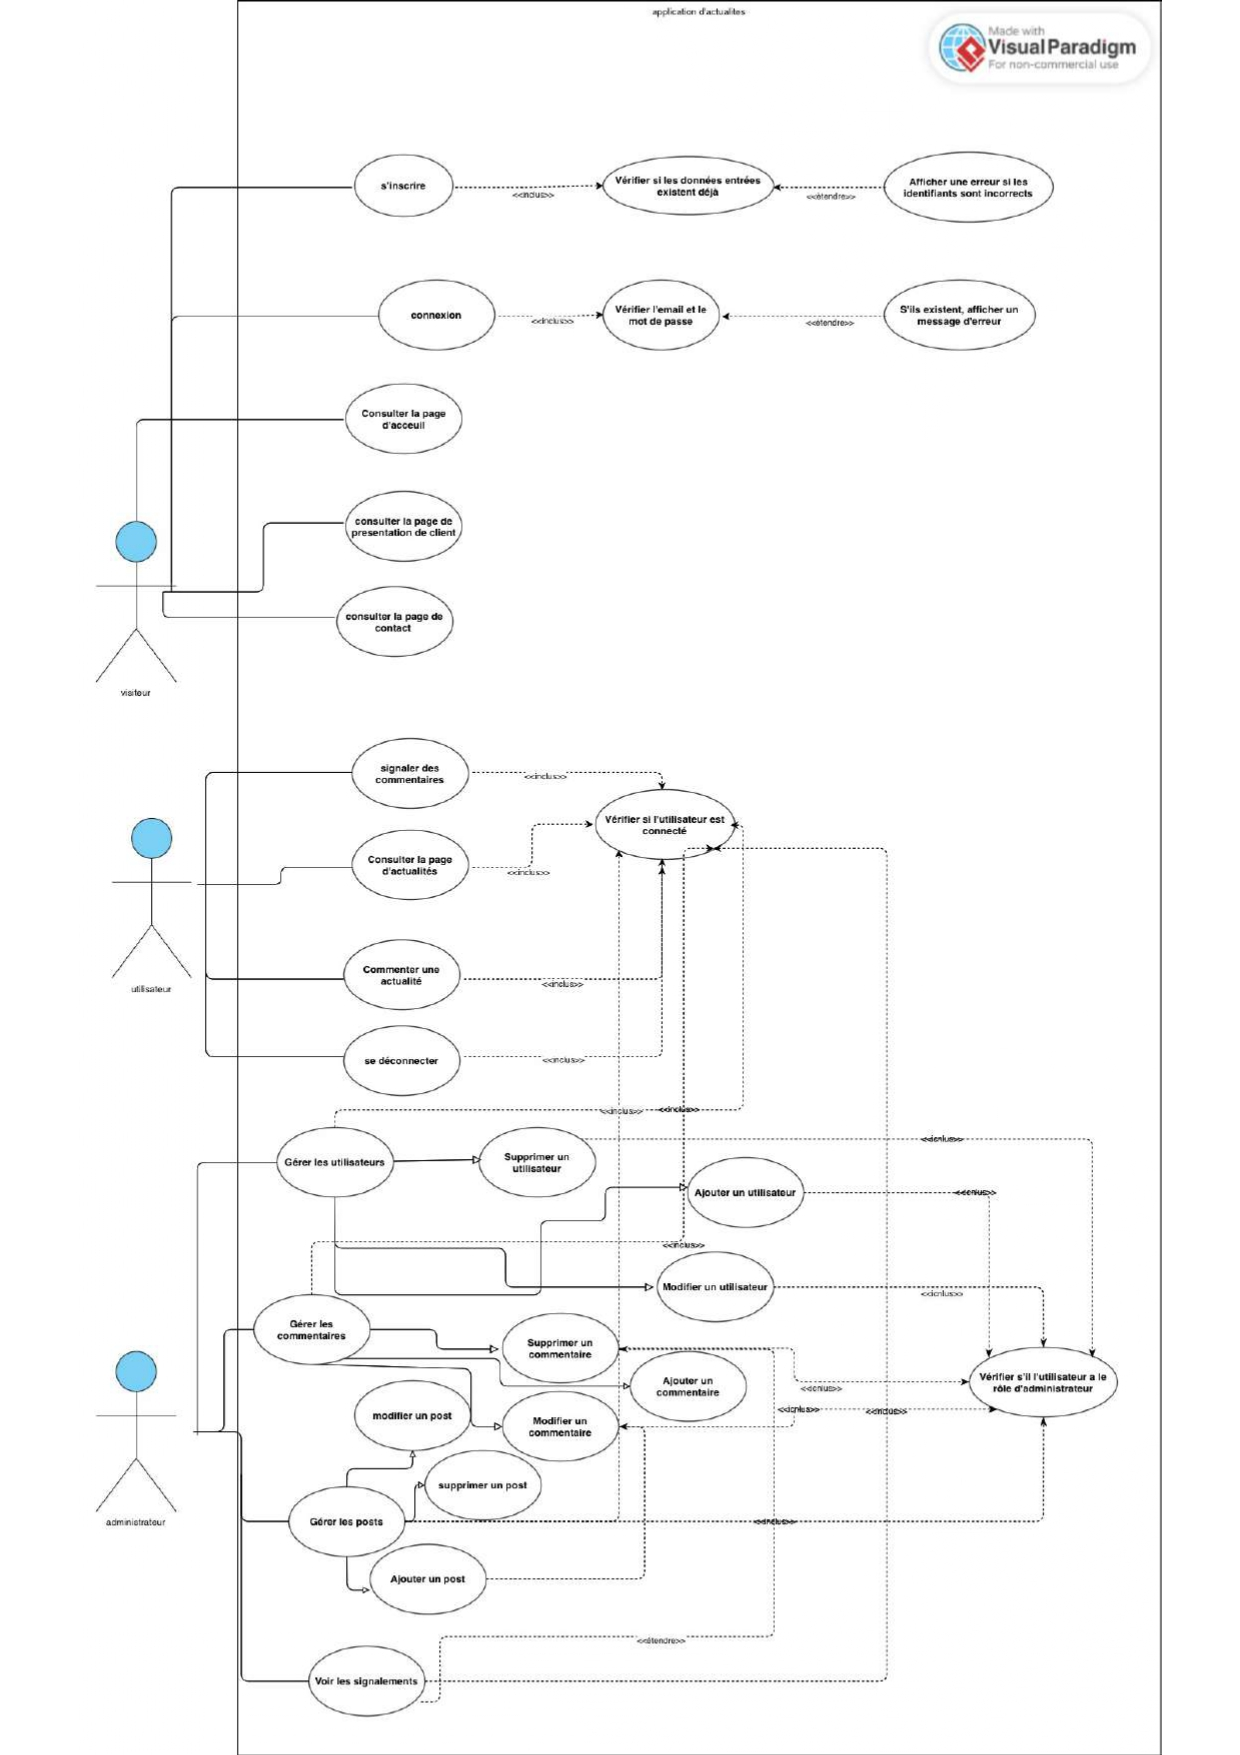
\includegraphics[scale=.65]{use_case.jpg}
		\caption{Diagramme des cas d'utilisation}
	\end{center}
\end{figure}	

\section{Diagramme de classes de la solution cible}

\begin{figure}[!h]
	\begin{center}
		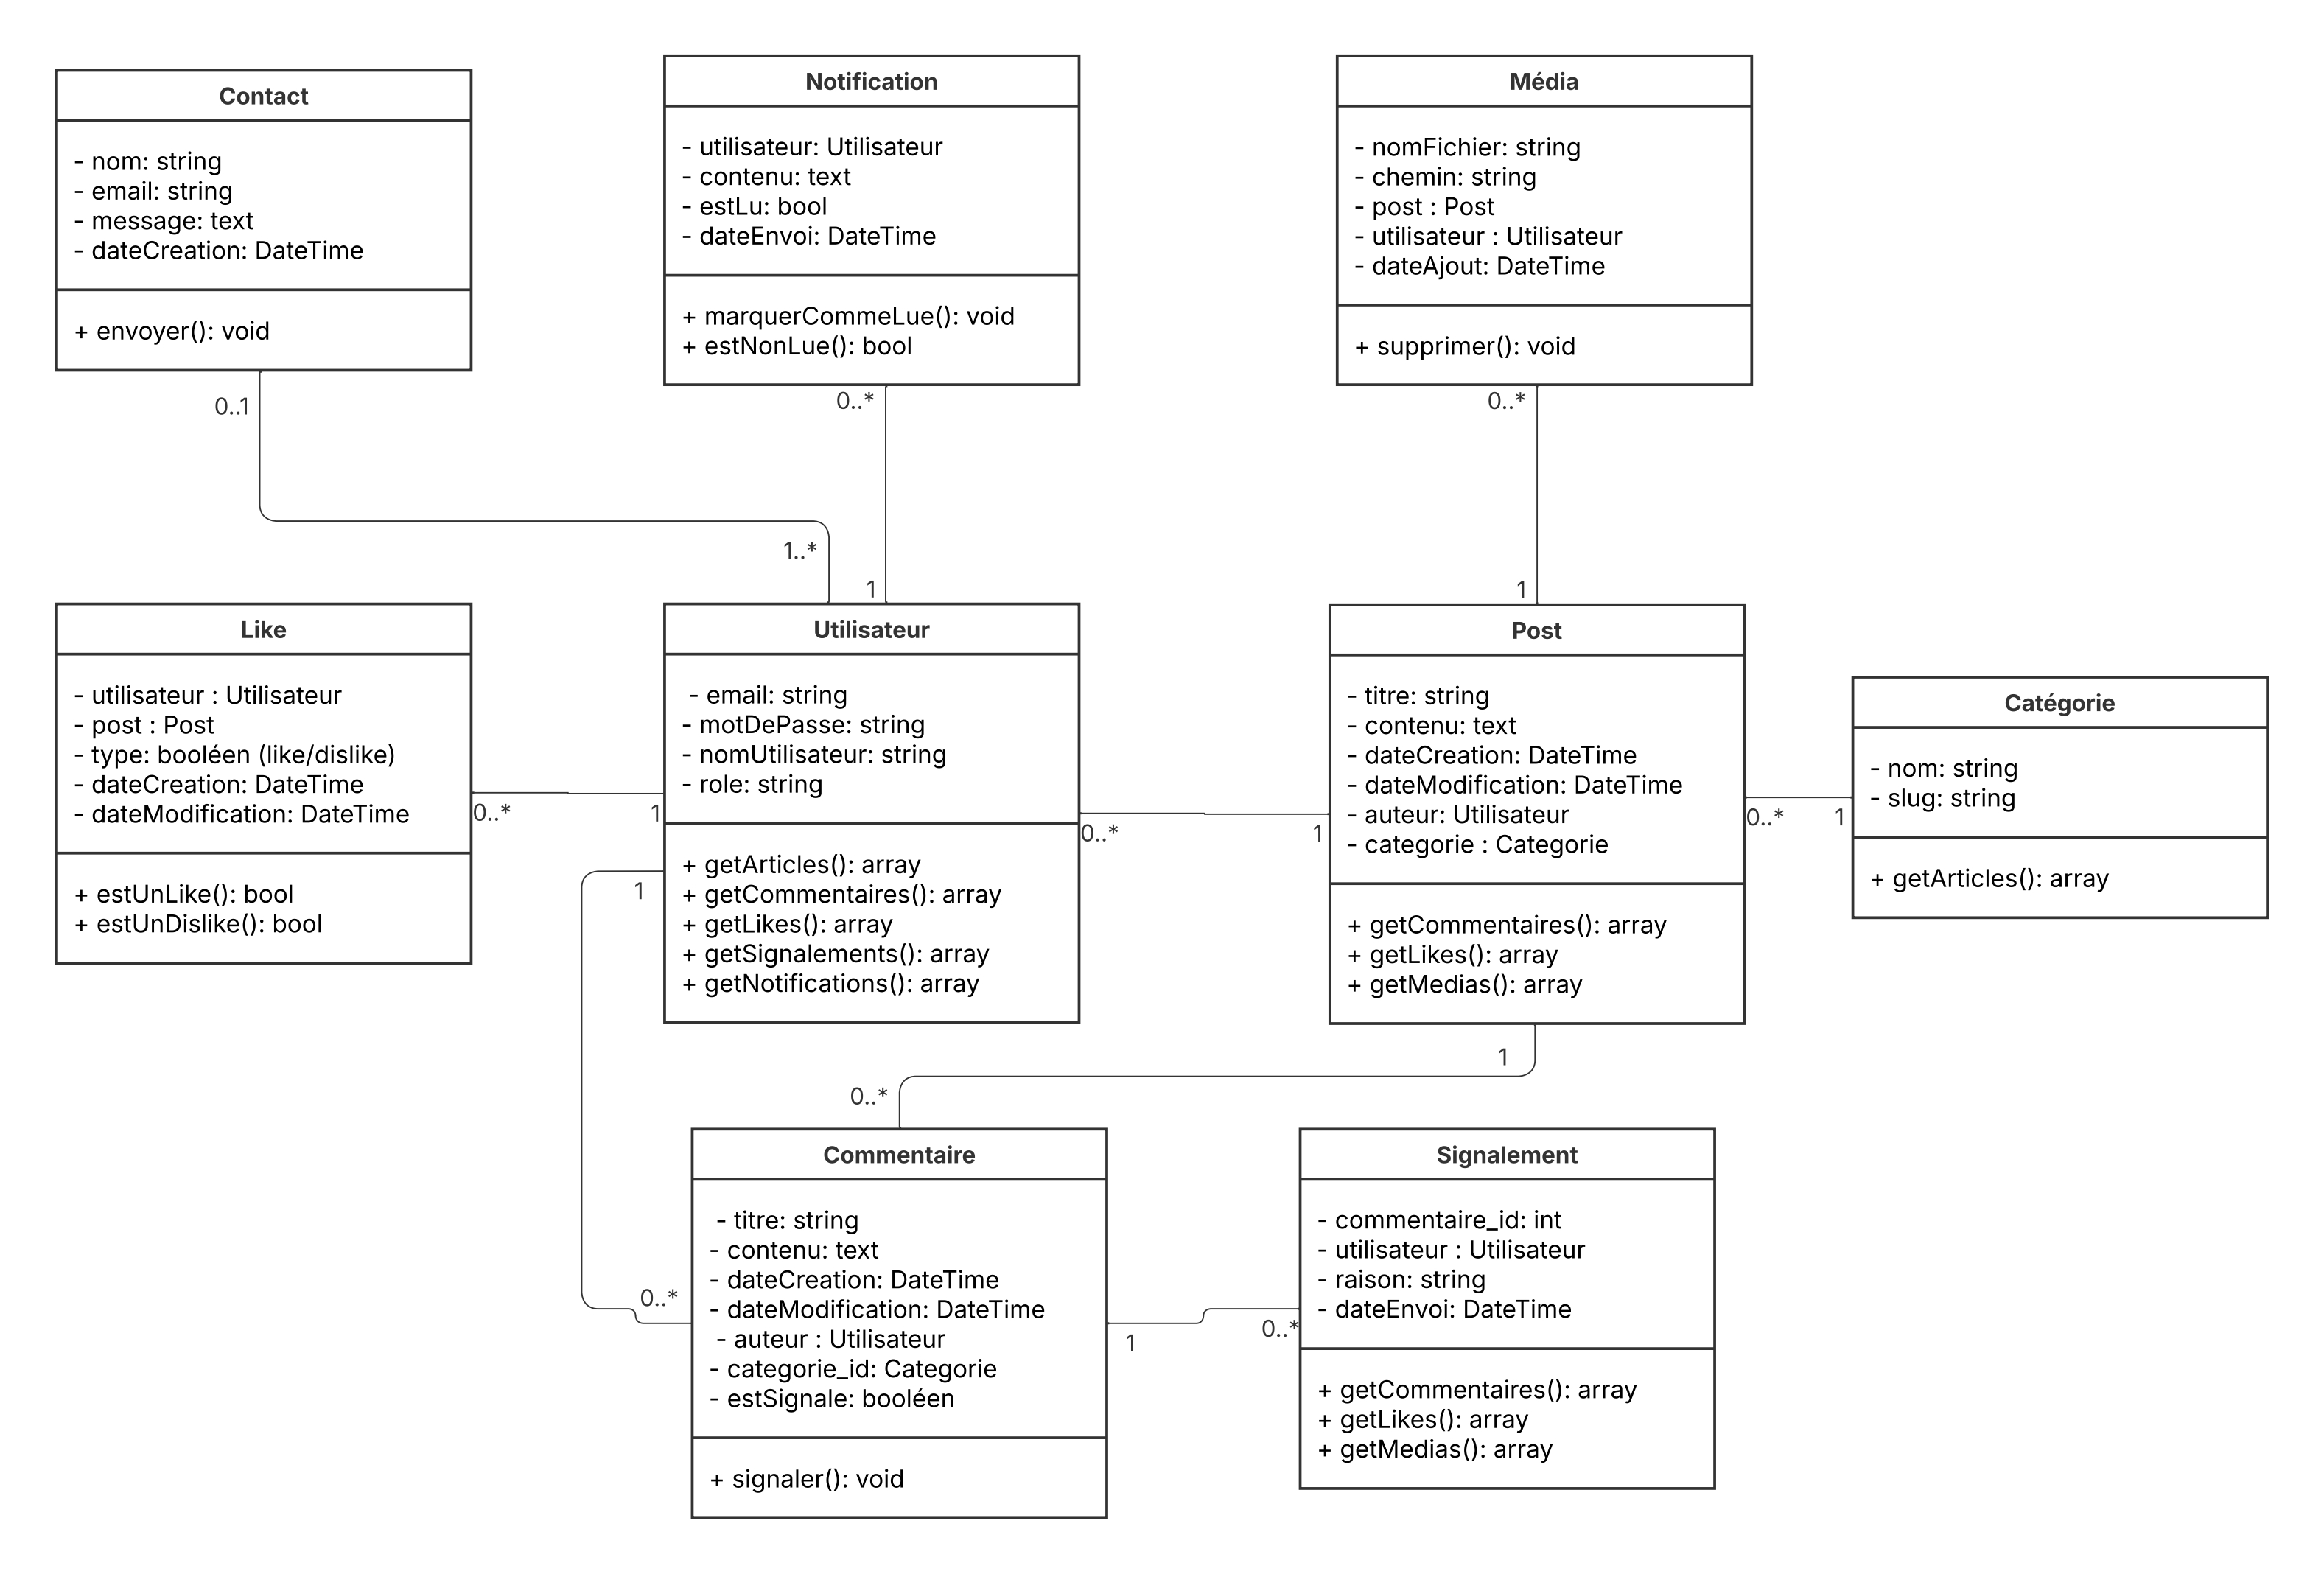
\includegraphics[scale=.65]{diagramme.jpg}
		\caption{Diagramme de classes}
	\end{center}
\end{figure}	

\newpage

\section{Spécifications fonctionnelles}


\subsection{Technologies utilisées}

\begin{itemize}
	\item[-] Le framework PHP Symfony, utilisant une version 7+ ;
	\item[-] Le moteur de templates Twig ;
	\item[-] Doctrine ORM pour gérer la base de données ;
	\item[-] Le framework CSS TailwindCSS ;
	\item[-] Le bundle EasyAdmin pour la partie administration du blog ;
	\item[-] Git et Github pour le versioning du code source du projet;
\end{itemize}

\subsection{Front Office}

\subsubsection{Page d'accueil}

    La page d’accueil affiche un aperçu graphique du site, ainsi que les 3 dernières actualités. \\
    
    Fonctionnalités :
    
    \begin{itemize}
    	\item[-] Affichage des 3 dernières actualités sous forme de titres cliquables, accompagnés d'un résumé ;
    	\item[-] Chaque actualité cliquée redirige vers une page dédiée à l’actualité ;
    	\item[-] Le design doit être épuré, responsive, avec un accent sur la lisibilité et l’esthétique ;
    \end{itemize}
        

\subsubsection{Page d’actualités}

    Cette page présente toutes les actualités publiées sur le site.\\
    
    Fonctionnalités :
    
        
	\begin{itemize}
    		\item[-] Liste des actualités avec une barre de recherche ;s
    		\item[-] Chaque actualité est affichée avec un titre, un extrait, et un lien vers sa page détaillée.
    \end{itemize}
        

\subsubsection{Page de chaque actualité}

    Page détaillée d'une actualité.\\
    
    Fonctionnalités 
    
    \begin{itemize}
    	\item[-] Affichage du titre, de la date de publication, du contenu complet de l'actualité.
    	\item[-] Section de commentaires où les utilisateurs peuvent poster des messages.
    	\item[-] Chaque commentaire peut être signalé par un utilisateur en cliquant sur un bouton "Signaler".
    \end{itemize}    

\subsubsection{Page de présentation du client}

    Présentation de l’entreprise ou du client qui a commandé le projet.\\
    
    Fonctionnalités :
    
    \begin{itemize}
    		\item[-] Texte de présentation ;
    		\item[-] Informations sur les services, l’histoire de l’entreprise, ou toute autre information pertinente ;
    \end{itemize}
        
        

\subsubsection{Page de contact}

    Formulaire de contact permettant aux utilisateurs de contacter l’entreprise.\\
    
    Fonctionnalités :
    
    \begin{itemize}
    		\item[-] Formulaire avec champs : nom, email, message.
    		\item[-] Envoi des informations par email au responsable de l'entreprise.
    \end{itemize}
       
       

\subsubsection{Page d’inscription}

    Permet aux utilisateurs de s’inscrire sur le site.\\

	Fonctionnalités :
    
    \begin{itemize}
    		\item[-] Formulaire avec champs : nom, email, mot de passe, confirmation du mot de passe.
    		\item[-] Validation des données (par exemple, vérifier si l’email est déjà utilisé, mot de passe suffisamment sécurisé).
    \end{itemize}

\subsubsection{Page de connexion}

    Permet aux utilisateurs de se connecter à leur compte.\\
    
    Fonctionnalités :
    
    \begin{itemize}
    		\item[-] Formulaire avec champs : email, mot de passe.
    		\item[-] Validation des données et affichage des erreurs (email ou mot de passe incorrect).
    		\item[-]  Redirection vers la page d'accueil une fois connecté.
    \end{itemize}
        
        

\subsection{Back Office}

Cette partie a été mise en place à l'aide du bundle EasyAdmin de Symfony. C'est un tableau de board d'administration qui permet d'accéder aux différentes fonctionnalités du back-office. \\

\subsubsection{Gestion des articles}

    Interface permettant à l'administrateur de gérer les actualités (articles).\\
    
    Fonctionnalités :
    
    \begin{itemize}
    		\item[-] Créer un nouvel article : champ titre, contenu, catégorie, date de publication ;
    		\item[-] Modifier les articles existants ;
    		\item[-] Supprimer un article ;
    		\item[-] Afficher la liste des articles publiés ;
    		\item[-] Possibilité de publier/dépublier un article (visibilité en front office).
    \end{itemize}
        
       
\subsubsection{Gestion des commentaires}

   	Interface permettant à l’administrateur de gérer les commentaires des utilisateurs.\\
   
    Fonctionnalités :
    \\
    \begin{itemize}
    		\item[-] Voir tous les commentaires associés à un article ;
    		\item[-] Approuver ou supprimer des commentaires ;
    		\item[-] Voir si un commentaire a été signalé ou non ;
    		\item[-] Afficher le nombre de commentaires signalés et leur contenu pour une gestion rapide.
    \end{itemize}
        .       

\subsubsection{Gestion des utilisateurs}

    Interface permettant à l’administrateur de gérer les utilisateurs inscrits sur le site.\\
    
    Fonctionnalités :
    
    \begin{itemize}
    		\item[-] Voir la liste des utilisateurs avec leurs informations: nom, email, role(s) ;
    		\item[-] Modifier ou supprimer des utilisateurs.
    \end{itemize}

\end{document}
